\documentclass[12pt, a4paper]{article}
\usepackage{pdfpages}
\usepackage{fancyhdr}
\usepackage{listings}
\usepackage{courier}
\usepackage{hyperref}

\pagestyle{fancy}
\fancyhf{}
\fancyhead[L]{Federico del Mazo - 100029}
\fancyhead[R]{21/12/2020}
\renewcommand{\headrulewidth}{0.4pt}
\fancyfoot[C]{\thepage}

\lstset{basicstyle=\footnotesize\ttfamily,breaklines=true}

\begin{document}
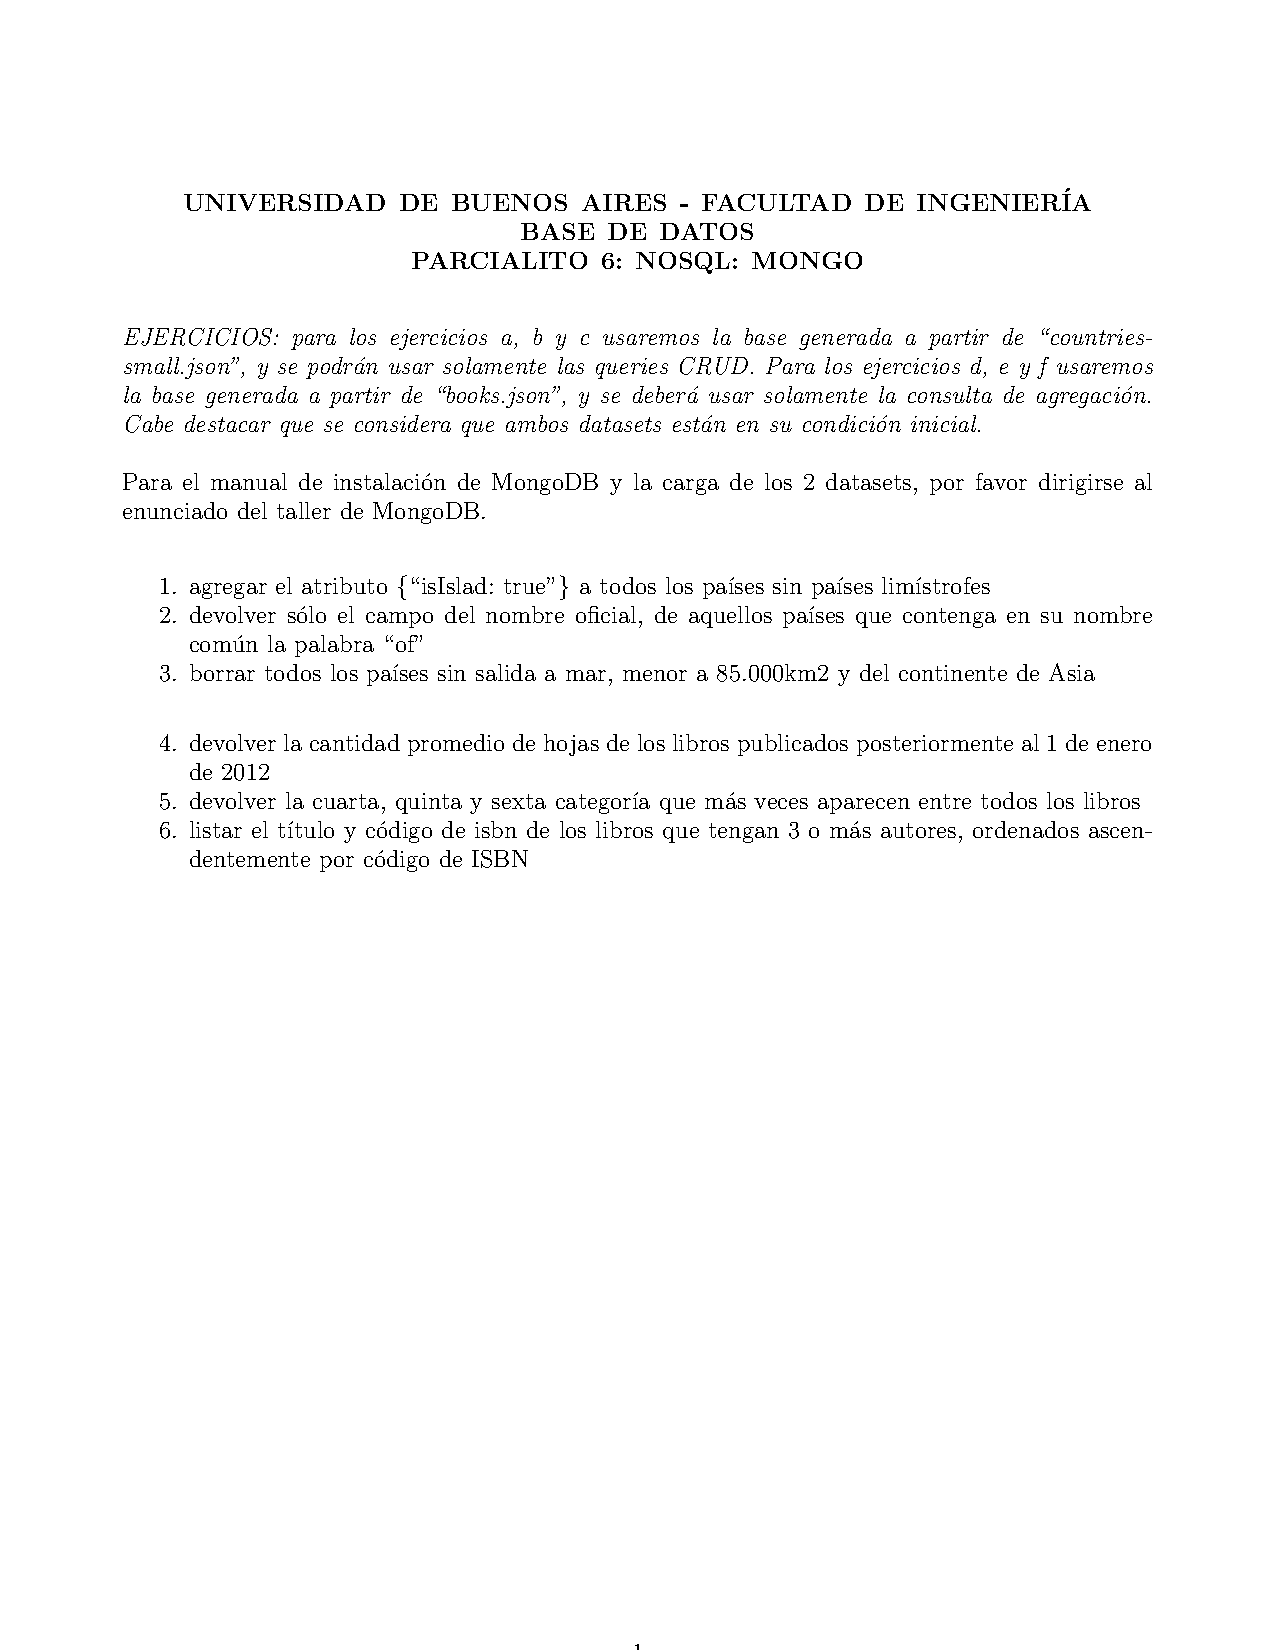
\includepdf{Parcialito6-Enunciado}
\setcounter{page}{1}

\begin{itemize}
\item agregar el atributo {“isIslad: true”} a todos los países sin países limítrofes
\begin{lstlisting}[frame=single]
db.countries.updateMany(
  { borders: { $size: 0 } },
  { $set: { isIsland: true } }
);
\end{lstlisting}

\item devolver sólo el campo del nombre oficial, de aquellos países que contengan en su nombre común la palabra “of”
\begin{lstlisting}[frame=single]
db.countries.find(
  {"name.common": /of/},
  {_id: 0, "name.official": 1}
)
\end{lstlisting}

\begin{lstlisting}[frame=shadowbox]
{name={official=Republic of the Congo}}
{name={official=Isle of Man}}
\end{lstlisting}

\item  borrar todos los países sin salida al mar, menores a 85.000km2 y del continente de Asia
\begin{lstlisting}[frame=single]
db.countries.deleteMany({
  landlocked: true,
  area: { $lt: 85000 },
  region: "Asia",
});
\end{lstlisting}

\begin{lstlisting}[frame=shadowbox]
{acknowledged=true, deletedCount=2}
\end{lstlisting}

\hrulefill

\item  devolver la cantidad promedio de hojas de los libros publicados posteriormente al 1 de enero de 2012
\begin{lstlisting}[frame=single]
db.books.aggregate([
  { $match: { publishedDate: { $gt: new Date("2012-01-01") } } },
  { $group: { _id: null, avgPageCount: { $avg: "$pageCount" } } },
  { $project: { _id: 0, avgPageCount: 1 } },
]);
\end{lstlisting}

\begin{lstlisting}[frame=shadowbox]
{avgPageCount=105.44871794871794}
\end{lstlisting}

\item  devolver la cuarta, quinta y sexta categoría que más veces aparecen entre todos los libros
\begin{lstlisting}[frame=single]
db.books.aggregate([
  { $unwind: "$categories" },
  { $group: { _id: "$categories", count: { $sum: 1 } } },
  { $sort: { count: -1 } },
  { $skip: 3 },
  { $limit: 3 },
  { $project: { count: 0, _id: 1 } },
]);
\end{lstlisting}

\begin{lstlisting}[frame=shadowbox]
{_id=Web Development}
{_id=Software Engineering}
{_id=Programming}
\end{lstlisting}

\item listar el título y código de ISBN de los libros que tengan 3 o más autores, ordenados ascendentemente por código de ISBN
\begin{lstlisting}[frame=single]
db.books.aggregate([
  { $addFields: { nauthors: { $size: "$authors" } } },
  { $match: { nauthors: { $gte: 3 } } },
  { $sort: { isbn: 1 } },
  { $project: { _id: 0, title: 1, isbn: 1 } },
]);
\end{lstlisting}

\begin{lstlisting}[frame=shadowbox]
{title=Portlets and Apache Portals}
{title=SNA and TCP/IP Enterprise Networking, isbn=131271687}
{title=Visual Object Oriented Programming, isbn=131723979}
{title=Planning and Managing ATM Networks, isbn=132621894}
{title=Making Sense of Java, isbn=132632942}
[...]
\end{lstlisting}

\end{itemize}
\end{document}
